\graphicspath{{chapters/images/01/}}

\chapter{\emph{Escherichia Coli} general informations}
\section{\emph{E. coli} genomics}
\emph{Escherichia Coli} is a Gram-negative, facultative anaerobic, rodshaped, coliform bacterium, it pertains to the phylum of proteobacteria and to the family of Enterobacteriaceae. It can be grown easily and inexpensively. It has got genome with a length between 4.5 - 4.7 M bases, including about 4000-5000 genes, and about seven ribosomal RNA operons. Only the 38\% of the genes of K-12 (one of the most studied bacterial strains of \emph{E. coli}) were experimentally identified, overall 40-50\% of the genes are to date without a known function.
The original \emph{E. coli} strain K-12 was obtained from a stool sample of a
diphtheria patient in Palo Alto, CA in 1922.

\subsection{\emph{E. coli} long-term evolution experiment}
The \emph{E. coli} long-term evolution experiment led by Richard Lenski is one of the longest evolutionary experiments ever made (search "\textit{The Longest-Running Evolution Experiment}"). The experiment started on 24th February 1988, and since that moment 12 populations of \emph{E. coli} have been cultivated in the same environment. After each day (corresponding to the time of development of approximately 7 generations), a portion of bacteria from each flask was introduced in a new one, and let proliferating in it. Every 500 generation, it has been saved a sample of the bacteria of each flask, in order to track the evolutionary changes made. Today the experiment is on-going, and researchers reached approximately the 66000th generation. The study suggests a series of conclusions, to cyte "long-term adaptation to a fixed environment can be characterized by a rich and dynamic set of population genetic processes, in stark contrast to the evolutionary desert expected near a fitness optimum" (Good et al 2017). In fact, despite of the fixed environment, some bacteria developed the capacity to aerobically grow on citrate, which is unusual in \emph{E. coli} (around generation 31,000) and developed complex mutation patterns.


\subsection{\emph{E. coli} strains}
\emph{E. coli} could be found as commensal strains, pathogenic strains, or environmental strains. The pathogenic strains could pertein to these categories (which are not exclusive): enteropathogenic (EPEC), enteroinvasive (EIEC), enterotoxigenic (ETEC), diffusely adherent (DAEC), adherent invasive (AIEC), shiga-toxin producing (STEC), enteroaggregative(EAEC), extraintestinal pathogenic (ExPEC). Resistances to antibiotics make even more difficult the process of categorization of \emph{E. coli}. 
In 2011 in Germany, an outbreak of Stx-EAEC was responsible of the death of some people. An efficient counter-measure was found by sequencing the genome of those bacteria. 

Shigella is \emph{E. coli} with shiga toxin. It had been an issue for toxonomists.

Most of the genes are on plasmids, circular, additional to chromosome, and can be moved easily horizontally. Plasmids between different strains can be moved in enterobacteriacae, this doesn't happen normally in other families.
Some \emph{E. coli} strains are even capable of causing tumors in humans: for example, colibactin-positive \emph{\emph{E. coli}} can cause colon and rectal cancer, by creating mutations which are responsable of the of the cancer onset.

several antigens can be used by taxonomists to cathegorize \emph{E. coli} strains. In particular there are the O, H, K antigens, respectively related to the somatic, the flagella and the capsule. O antigens are 171, Ks are 80 and Hs are 56.

\subsection{PanPhlAn - strain detection and characterization}

Pangenome-based Phylogenomic Analysis (PanPhlAn) is a strain-level metagenomic profiling tool
for identifying the gene composition and in-vivo transcriptional activity of individual strains in metagenomic samples. PanPhlAn’s ability for strain-tracking and functional analysis of unknown pathogens makes it an efficient tool for culture-free infectious outbreak epidemiology and microbial population studies (\href{http://segatalab.cibio.unitn.it/tools/panphlan/}{PanPhlAn reference}). This tool was for example used to study the strain responsible of an outbreak in Germany in 2011. This strain was a shiga-toxigenic Escherichia coli (STEC), and the study was conducted by Loman and collegues in 2013.
This method outlasted the traditional one.


sequencing means generally to sequence everything, it's normally difficult where to find it, although in \emph{\emph{E. coli}} is quite easy to understand the provenience.
from all the world, populating diversity of \emph{\emph{E. coli}}, every time we sample we find points which are different from the reference genomes.
points overlapping are people living together and share bacterias


\subsection{Genomes of \emph{E. coli}}

In the genome of \emph{E. coli} strains, it is possible to distinguish:

\begin{itemize}
    \item \textbf{Core genome}: the set of all genes shared by all membrers of a bacterial species, it includes 1000 up to 3000 genes.
    \item \textbf{Accessory or dispensable genome}: the set of genes present in some but not all genomes within the same bacterial species. found on a single strain or in a subset of strains. 
    \item \textbf{Pangenome}: core genome + accessory genome. set of all the genes foundable in the species strains. It is said to be \textit{\textbf{"closed"}} when pangenome size tends to a maximum as number of genomes increases, instead it is \textit{\textbf{"open"}} when pangenome keeps increasing as you add new genomes
\end{itemize}


Sequencing more organism of the same species means to lower the amount of genes in the core genome and augment the numer of those in the pan-genome (figure \ref{corepangenome}). 
Because of technical problems the probability of getting a gene and not forget it is different from 0, so why probably the sequencing of other genomes would lead technically to a plummet to 0 of the pangenome. With some mathematical formulations we can predict a more probable plateau (Rasko David 2008). 

\begin{figure}[h]
\caption{Core- and pan- genome of \emph{E. coli}}\label{corepangenome}
\centering
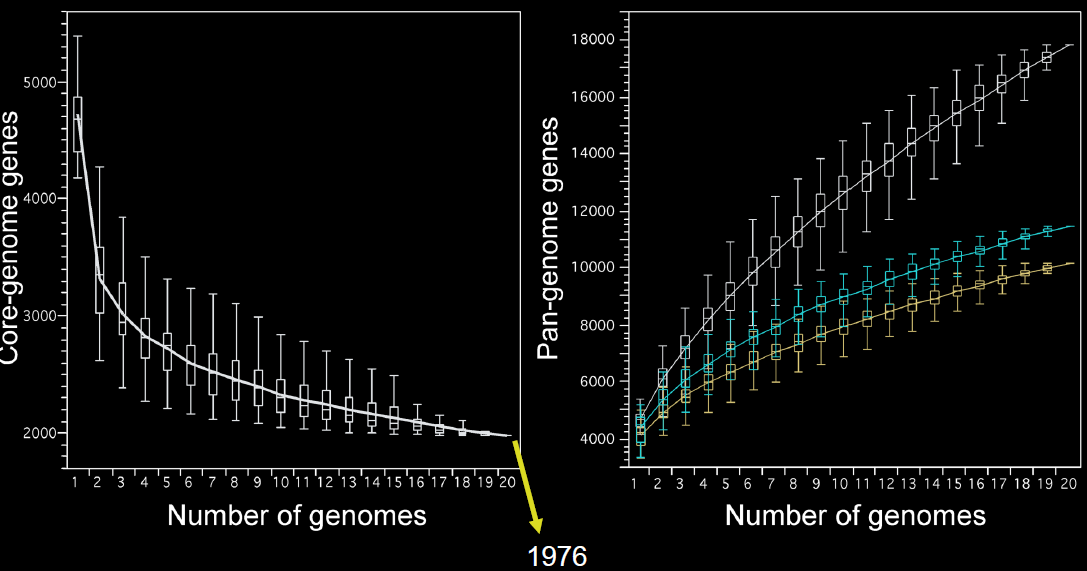
\includegraphics[width=0.6\textwidth]{EcoliCorePanGenome}
\end{figure}


\begin{figure}[h]
\caption{It can be seen that 51\% of the genes are strain specific, and the other are shared between 2 to 20.  of \emph{E. coli}}
\centering
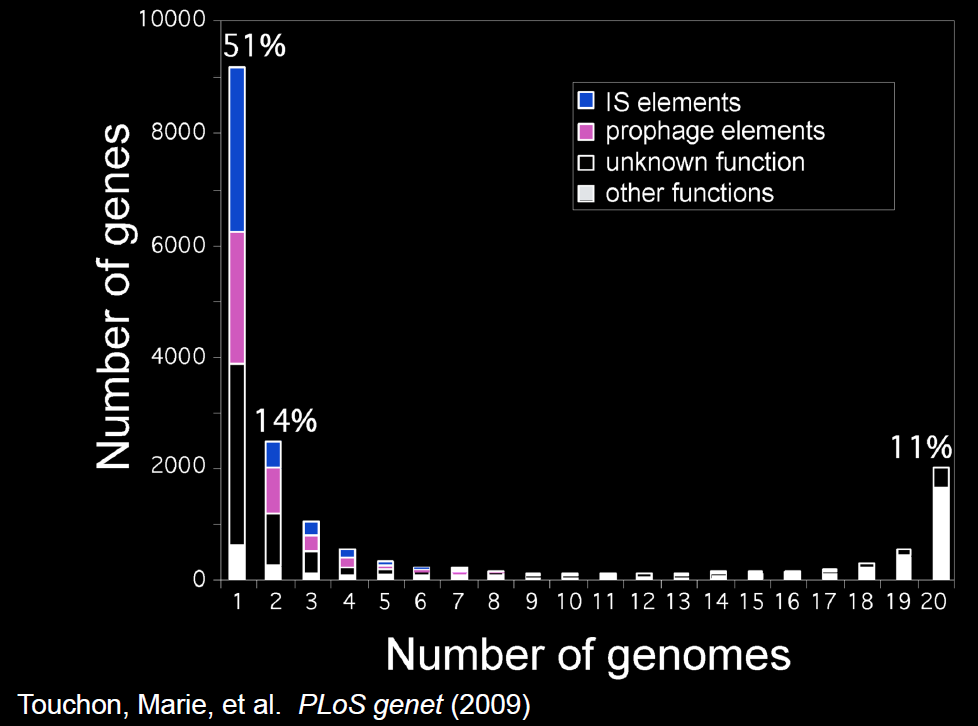
\includegraphics[width=0.6\textwidth]{genesSharedDifferentGenomes}
\end{figure}



\begin{figure}[h]
\caption{A different definition of orthologous genes can modify the number of pan genes of a species. }
\centering
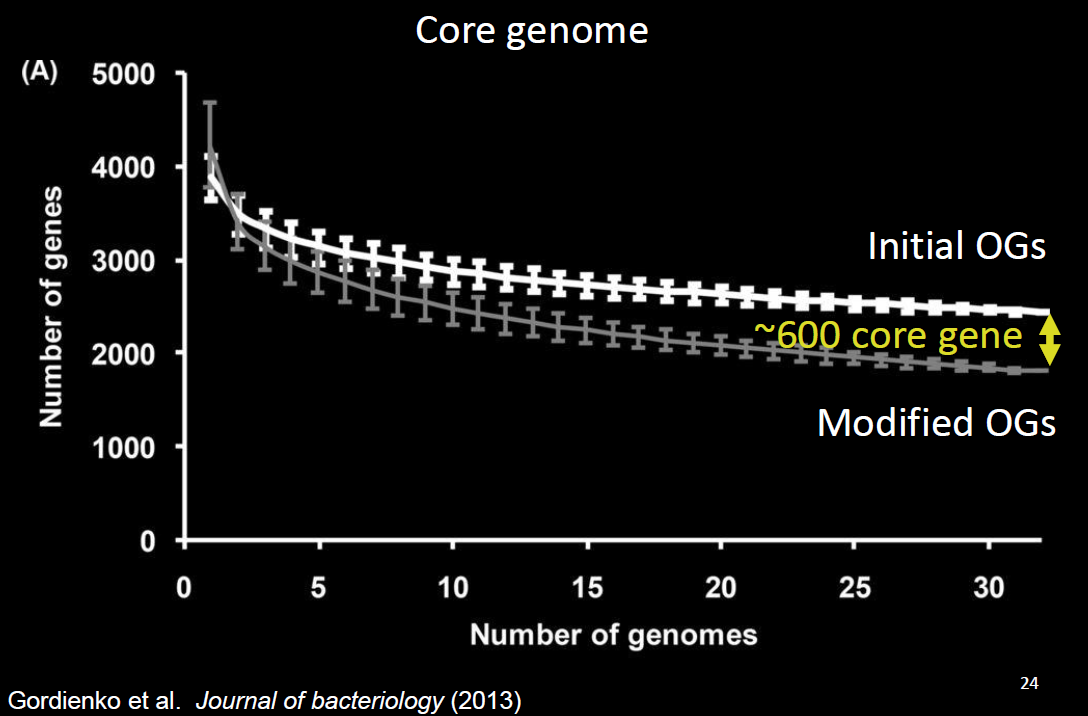
\includegraphics[width=0.6\textwidth]{orthologGenes}
\end{figure}



\begin{figure}[h]
\caption{we predict a core genome size of 3079 genes for extraintestinal pathogenic \emph{E. coli}}
\centering
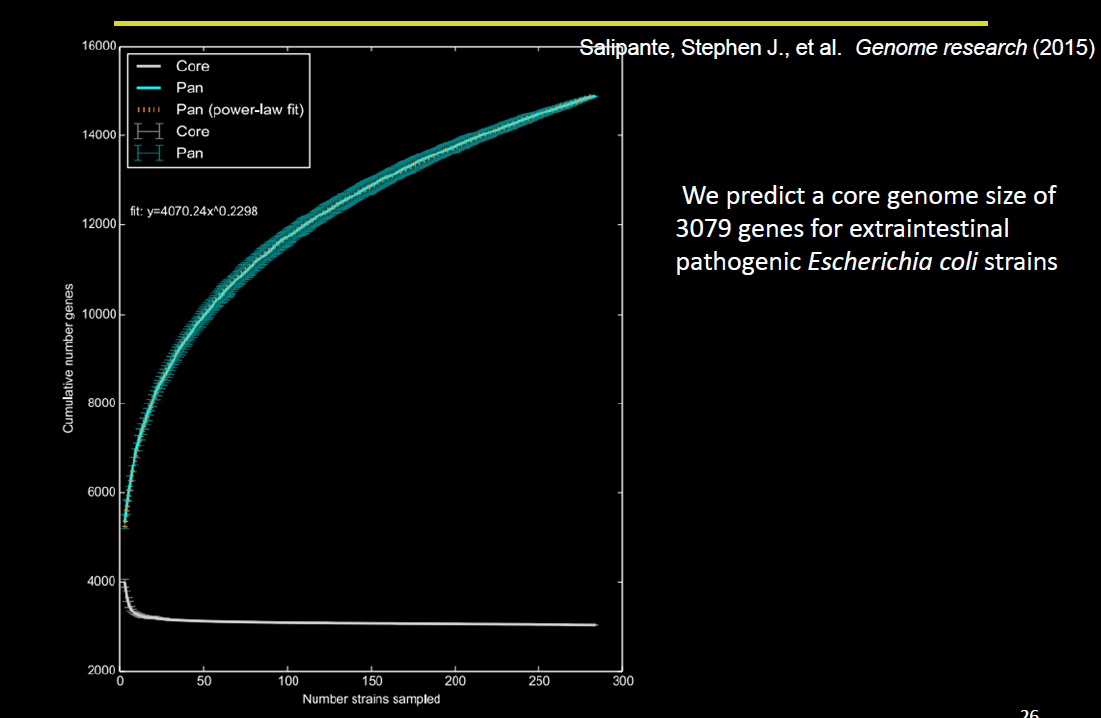
\includegraphics[width=0.6\textwidth]{coreGenomePredict}
\end{figure}

each \emph{E. Coli} genome contains in a balanced way genes of the core genome and of the pan genome, for a total amount of genes correspondant to about 4700 genes (figure \ref{balancepancore}). Core genomes' genes are responsible of some basic cellular functionalities and utilities to survive environent, while instead elements of the pangenome are quite usually specific to the single strains, they are not always functionally well known. 

\begin{figure}[h]
\caption{Balance between genes of the core- and of the pan-genome}\label{balancepancore}
\centering
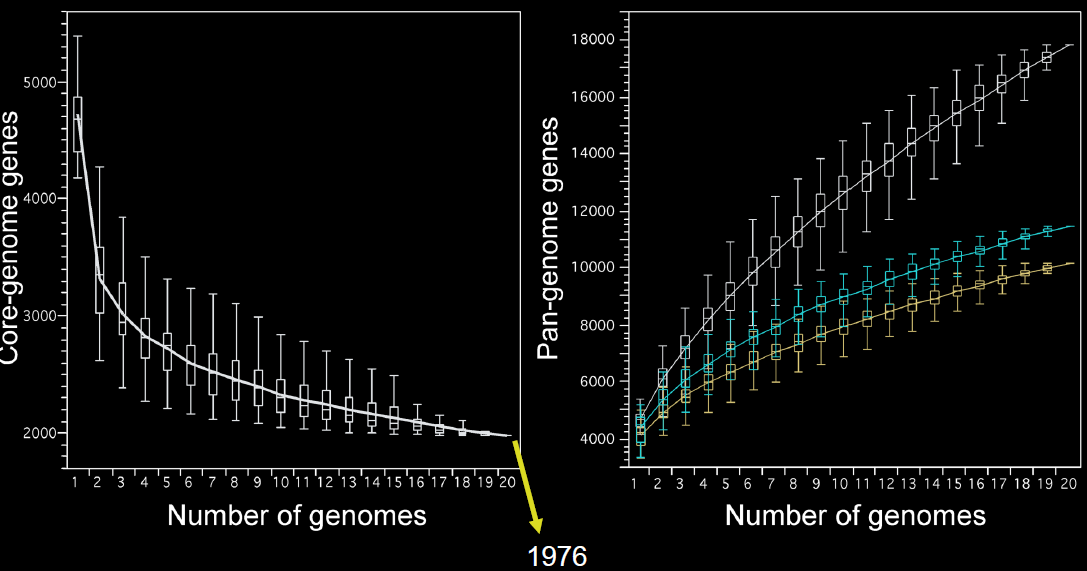
\includegraphics[width=8cm]{corePanGenEcoli}
\end{figure}

ratios of the pan-genome and the core-genome are not equal in other
organisms behave differently.